\fakesection{Simuleren van Sparen en Beleggen}

\begin{center}
\textit{De broncode bevindt zich in de \texttt{src} folder. Het algemene script (\texttt{src/s0216676\_script}) is opgedeeld in secties, \'e\'en per opgave. Elke opgave wordt hieronder afzonderlijk beantwoord. Aan het einde van elk antwoord wordt (indien nodig) de broncode weergegeven.}
\end{center}

%%%
%%%
%%%

\fakesubsection{Opdracht 1}

Hier is een implementatie :

\begin{lstlisting}
function [yield, invested, value] = s0216676_simulateSavingInvesting(budget, rate, months)
    value = repelem(budget * 1.02 .^ (0:floor(months/12)), 1, 12); 
    invested = sum(value(1:months));
    for j = 13:12:months % Consider each month of january
    	win = sum(value(j-12:j-1) .* (((12:-1:1)/12) * (rate/100))); % Calculate savings
    	value(j) = value(j) + (win - 0.15 * (win > 980) * (win - 980));
        value(j-12:j) = cumsum(value(j-12:j)); % Accumulate sums
    end
    value = value(1:months); value(j:end) = cumsum(value(j:end));
    yield = value(months) / invested - 1;
end
\end{lstlisting}

%%%
%%%
%%%

\fakesubsection{Opdracht 2}

Het resultaat van de gegeven code is te zien in figuur \ref{fig:op2}. De totale investering bedraagt zo'n 96091 euro. De relatieve winsten bedragen 5.46\%, 11.34\%, 23.34\% en 50.82\%.

\vspace{0.3cm}
\begin{figure}[h]
\centering
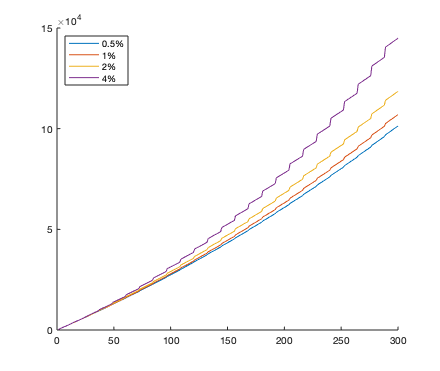
\includegraphics[width=0.5\textwidth]{res/op2.png}
\caption{Simulatie van spaarrekeningen met verschillende rentevoeten.}
\label{fig:op2}
\end{figure}

%%%
%%%
%%%

\fakesubsection{Opdracht 3}




